\documentclass[11pt,utf8]{article}
\usepackage[utf8]{inputenc}
\usepackage[francais]{babel}
\usepackage{graphicx}
%\usepackage[latin1]{inputenc}
%\usepackage[french]{babel}
\usepackage{amsmath,amssymb,amsfonts}
\usepackage{hyperref}
\hypersetup{
     colorlinks   = true,
     citecolor    = gray
} 
 \usepackage{amsmath,scalerel}
\usepackage{textcomp}
\usepackage{enumerate}% http://ctan.org/pkg/enumerate

\DeclareMathOperator*{\Bigcdot}{\scalerel*{\cdot}{\bigodot}}


\usepackage{colortbl,booktabs}
\usepackage{listings}
\usepackage{pgfplots,pgfplotstable}
\usepackage{xspace}
\usepackage{tikz}
\usetikzlibrary{arrows,patterns,plotmarks,shapes,snakes,er,3d,automata,backgrounds,topaths,trees,petri,mindmap}


\definecolor{lbcolor}{rgb}{0.95,0.95,0.95}
\definecolor{cblue}{rgb}{0.,0.0,0.6}

\newcommand{\Air}{\text{\textsc{Air}}\xspace}
\newcommand{\PCB}{\text{\textsc{PCB}}\xspace}
\newcommand{\IC}{\text{\textsc{IC}}\xspace}
\newcommand{\ICs}{\text{\textsc{ICs}}\xspace}

\newcommand{\OPUS}{\textsc{OPUS}\xspace}
\newcommand{\FF}{\textsc{Freefem++}\xspace}
\newcommand{\COMSOL}{\textsc{Comsol}\xspace}
\newcommand{\COMSOLUJF}{\textsc{Comsol(UJF)}\xspace}
\newcommand{\COMSOLEADS}{\textsc{Comsol(EADS)}\xspace}
\newcommand{\Feelpp}{\textsc{Feel++}\xspace}
\newcommand{\GMSH}{\textsc{Gmsh}\xspace}
\newcommand{\BOOST}{\textsc{Boost}\xspace}

\newcommand{\UJF}{\textsc{UJF}\xspace}
\newcommand{\EADS}{\textsc{EADS}\xspace}

\newcommand{\vect}[1]{\ensuremath{\mathbf{#1}}\xspace}


\definecolor{Lightgray}{rgb}{0.85, 0.85, 0.85}

\usepackage{filecontents,listings}
\lstset{language=c++,showspaces=false,showstringspaces=false,captionpos=t,literate={>>}{\ensuremath{>>}}1,mathescape}
\lstset{basicstyle=\small\bf\ttfamily}
\lstset{lineskip=-2pt}

%\lstset{emph={inline},emphstyle=\color{red}\bfseries}

\definecolor{cgreen}{rgb}{0.,0.6,0.0}

\definecolor{violet}{rgb}{0.5,0,0.5}
\definecolor{vertfonce}{rgb}{0.,0.5,0.}
\definecolor{rouge}{rgb}{0.5,0.,0.}
\definecolor{bleu}{rgb}{0.,0.,1}
\definecolor{orange}{rgb}{1,0.5,0}
\lstset{keywordstyle=\color{red}\bfseries}
\lstset{
emph={form,form1,form2,integrate,on,grad,gradt,dot,id,dx,dy,dz,idt,dxt,dyt,dzt,idv,dxv,dy,dzv,gradv,div,divt,divv,dn,jump,trans,vec,cst,
  project,P,Px,Py,Pz,one,oneX,oneY,oneZ,hFace,N,Nx,Ny,Nz,sin,cos,min,max,abs,pow,chi,exp,LinearForm,BilinearForm,MixedLinearForm,MixedBilinearForm,
  FESpace,MixedFESpace,integrate,project,addCL},emphstyle=\color{bleu},
emph={[2]\_space,\_range,\_expr,\_quad,\_quad1,\_test,\_trial,\_matrix,\_vector,\_solution,\_element,\_rhs,\_rowstart,\_colstart,\_block,
  \_pattern,\_pattern\_block,\_domainSpace,\_imageSpace,\_mesh,\_name,\_partitions,\_worldcomm,\_worldscomm,
  \_type,\_marker1,\_marker2,\_marker3,\_marker4,\_marker5,\_marker6,\_marker7,\_marker8,\_markerAll,\_argc,\_argv,\_desc},emphstyle={[2]\color{violet}\bfseries},
emph={[3]elements,markerName,boundaryfaces,markedfaces,\_Q,solve, newMatrix,newVector,newZeroMatrix,newZeroVector,
  newBlockMatrix,newBlockVector,localize,element,apply,createMesh,localSize,subWorldComm,transpose,setMarker,add,save,
  dirichlet\_vec,neumann\_scal,updateTime,exportResults,updateBdf,init,FluidMechanics}, emphstyle={[3]\color{rouge}\bfseries},
emph={[4]Backend,BlocksVector,BlocksSparseMatrix,BlocksStencilPattern,Blocks,opInterpolation,FunctionSpace,Lagrange,bases,Pch,unitSquare,WorldComm,
  Mesh,Simplex,Node,Rectangle,Quadrangle,Circle,AppliManagement,Environment,feel\_options,exporter},emphstyle={[4]\color{orange}\bfseries},
emph={[5]size\_type,uint16\_type},emphstyle={[5]\color{red}\bfseries},
emph={[6]GeoTool,vf,cl},emphstyle={[6]\color{cyan}\bfseries}
}


\lstset{commentstyle=\ttfamily\color{cgreen}}
\lstset{numberstyle=\tiny}
\lstset{backgroundcolor=\color{lbcolor},rulecolor=}

\lstset{frame=single,framerule=0.5pt}
\lstset{belowskip=\smallskipamount}
\lstset{aboveskip=\smallskipamount}
\lstset{includerangemarker=false,rangeprefix=\/\/\#\ ,% curly left brace plus space
  rangesuffix=\ \#}


%--------dimension
\textwidth 185 true mm
\textheight 220 truemm
\voffset -15 true mm
\hoffset -18 true mm

\def \x  {\textbf x}
\def \n  {\textbf n}
\def \cT {{\cal T}}


% above is the preamble
\title{INTERNSHIP REPORT}
\author{PREPARED BY :\\ Kyoshe Winstone\\University of Strasbourg\\STRASBOURG}

\begin{document}

\begin{center}
\textbf{{\large INTERNSHIP REPORT} }\\ % \\ = new line
\end{center}
\begin{center}
\copyright 2015 by Kyoshe Winstone \\
\end{center}

\begin{center}
MASTER 1 CSMI\\
\end{center}
\begin{center}
JUly 17, 2015

\end{center}
\begin{center}
 
\includegraphics[width=10cm,height=10cm]{p1}
 \end{center}
 \begin{center}
 
\section*{FEEL++  }
\begin{center}
\textbf{{\large  THE FEELPP-TUTORIAL} }\\ % \\ = new line
   \end{center}
\label{weekly report of the internship}

\end{center}
\newpage

\section{Introduction}
Feel++ is a unified C++ implementation of Galerkin methods (finite and spectral element methods) in 1D, 2D And 3D to solve partial differential equations.\\
For this part of the project,we concentrate much on  Checking and reproducing the Step by Step tutorial of the feels project.
The aim here is to read and understand the step by step tutorial and finally to be able to reproduce the tutorial, by making all necessary modifications and comments.\\ 
We also omit all unnecessary info from the tutorial.


\section{\textbf{Setting and compiling feelpp source codes to generate the necessary  files :}}
\begin{enumerate}[i]
\item log files
\item confi files
\item Expected Results (mesh)
\end{enumerate}
To compile our codes, we simply use the command line 
 \begin{lstlisting}
make feelpp_doc_<appname>.
 \end{lstlisting}
For instance,  for myapp
 \begin{lstlisting}
make feelpp_doc_myapp
 \end{lstlisting}
 We can also use parallelism to compile our source code, for example 
\begin{lstlisting}
make -j 10 feelpp_doc_<appname>
\end{lstlisting}


\textbf{NOTE :} 
To visualize the generated mesh, we can use the following line command :
\begin{lstlisting}
ssh -Y $\cdot \cdot \cdot$ [ $\cdot \cdot \cdot$] gmsh theFile.{msh,geo}
\end{lstlisting}
Feel++ uses \textbf{cmake} as its build system.\\
\textbf{It is not allowed to build the library in the source directory} : The best way is to have a directory (FEEL for example) in which you have: 
 \begin{center}
 \begin{lstlisting}

 ls FEEL feel/ // Sources feel.opt/ // Build directory 
 \end{lstlisting}
 \end{center}

 where feel is the top directory where the source have been downloaded, using git or trackballs.
Once CMake has done its work, you are now able to compile the library with:\\
 \begin{center}
 \begin{lstlisting}

  make
 
 \end{lstlisting}
  \end{center}
You can speed up the compilation process, if you have a multicore processor. To do so, you have to specify the number of parallel jobs make will be allowed to spawn by using the -j flag:

   \begin{center}
 \begin{lstlisting}
  make -j <nbjobs>
   \end{lstlisting}
  \end{center}
  
  \newpage
 We can find generated files after Feel++ compilation in following directories :
\begin{center}
 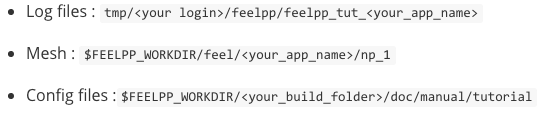
\includegraphics{f1}
 \end{center}
 
 We continue to make all necessary adjustements to the tutorial.

\newpage
\section{REFERENCES}
\begin{enumerate}[1]
\item \href{http://www.stack.nl/~dimitri/doxygen/manual/docblocks.html.}{DOXYGEN MANUAL}   
\item \href{http://www.cmake.org/cmake/help/v3.0/command/option.html}{CMAKE COMMANDS}
\item \href{http://gl.developpez.com/tutoriel/outil/makefile/}{MAKEFILE TUTORIAL}
 \item \href{http://www.cmake.org/cmake-tutorial/}{CMAKE TUTORIAL}
\end{enumerate}
\end{document}